
\documentclass[journal]{IEEEtran}
% \documentclass[conference]{IEEEtran
\IEEEoverridecommandlockouts
% The preceding line is only needed to identify funding in the first footnote. If that is unneeded, please comment it out.
\usepackage{cite}
\usepackage[margin=1in]{geometry}
\usepackage{amsmath,amsthm,amssymb}
\usepackage{mathtools}
\usepackage{hyperref}
\usepackage{scrextend}
\usepackage{algorithmic}
\usepackage{graphicx} 
\graphicspath{{./figures/}{../png/} }
\usepackage{subfig}
\usepackage[para,online,flushleft]{threeparttable}
\usepackage{wrapfig}
\def\BibTeX{{\rm B\kern-.05em{\sc i\kern-.025em b}\kern-.08em
    T\kern-.1667em\lower.7ex\hbox{E}\kern-.125emX}}

% This is to include code
\usepackage{listings}
\usepackage{xcolor}
\definecolor{dkgreen}{rgb}{0,0.6,0}
\definecolor{gray}{rgb}{0.5,0.5,0.5}
\definecolor{mauve}{rgb}{0.58,0,0.82}
\lstdefinestyle{Python}{
    language        = Python,
    basicstyle      = \ttfamily,
    keywordstyle    = \color{blue},
    keywordstyle    = [2] \color{teal},
    stringstyle     = \color{green},
    commentstyle    = \color{red}\ttfamily}

\newcommand{\N}{\mathbb{N}}
\newcommand{\Z}{\mathbb{Z}}

\newenvironment{theorem}[2][Theorem]{\begin{trivlist}
\item[\hskip \labelsep {\bfseries #1}\hskip \labelsep {\bfseries #2.}]}{\end{trivlist}}
\newenvironment{lemma}[2][Lemma]{\begin{trivlist}
\item[\hskip \labelsep {\bfseries #1}\hskip \labelsep {\bfseries #2.}]}{\end{trivlist}}
\newenvironment{exercise}[2][Exercise]{\begin{trivlist}
\item[\hskip \labelsep {\bfseries #1}\hskip \labelsep {\bfseries #2.}]}{\end{trivlist}}
\newenvironment{reflection}[2][Reflection]{\begin{trivlist}
\item[\hskip \labelsep {\bfseries #1}\hskip \labelsep {\bfseries #2.}]}{\end{trivlist}}
\newenvironment{proposition}[2][Proposition]{\begin{trivlist}
\item[\hskip \labelsep {\bfseries #1}\hskip \labelsep {\bfseries #2.}]}{\end{trivlist}}
\newenvironment{corollary}[2][Corollary]{\begin{trivlist}
\item[\hskip \labelsep {\bfseries #1}\hskip \labelsep {\bfseries #2.}]}{\end{trivlist}}

\hyphenation{op-tical net-works semi-conduc-tor}

%% For our reference part
%\makeatletter
%\def\bstctlcite{\@ifnextchar[{\@bstctlcite}{\@bstctlcite[@auxout]}}
%\def\bstctlcite[#1]#2{\@bsphack\@for\@citeb:=#2\do{%
%\edef\@citeb{\expandafter\@firstofone\@citeb}%
%\if@filesw\immediate\write\csname #1\endcsname{\string\citation{\@citeb}}\fi}
%\@esphack}
%\makeatother

\begin{document}
%\bstctlcite{IEEEexample:BSTcontrol}

% --------------------------------------------------------------
%                         Start here
% --------------------------------------------------------------

\title{Evaluating the Impact of Image Normalization on Automatic Segmentation of Brain Regions}

\author{\IEEEauthorblockN{Thomas Buchegger} \IEEEauthorblockA{\textit{University of Bern,}}
\and \IEEEauthorblockN{Carolina Duran} \IEEEauthorblockA{\textit{University of Bern,}}
\and \IEEEauthorblockN{Stefan Weber,} \IEEEauthorblockA{\textit{University of Bern}}
\thanks{All authors contributed equally. Biomedical Engineering, University of Berne in Switzerland. Author's E-Mails:}%
\thanks{thomas.buchegger@students.unibe.ch}%
\thanks{carolina.duran@students.unibe.ch}%
\thanks{stefan.weber1@students.unibe.ch}}

\markboth{Medical Image Analysis Lab, January~2021}%
{}
\maketitle
%\pagestyle{plain}
\newpage


% --------------------------------------------------------------
% Abstract
% --------------------------------------------------------------

\begin{abstract}
	This paper addresses the question whether image normalization leads to better results in brain region segmentation. To answer this question,
	we used a random forest classifier and compared six different normalization methods with each other and the ground truth segmentation. The evaluation of the segmentation performance
	of our algorithm on T1- and T2-weighted MRI volumes shows no significant improvement compared to no normalization. 
\end{abstract}
\hfill January 03, 2021

% --------------------------------------------------------------
% Introduction
% --------------------------------------------------------------

\section{Introduction}

	Every year, an estimated 13.8 million patients worldwide require a neurological surgery. The majority of neurosurgical care include traumatic brain injuries, tumors, stroke-related conditions and epilepsy. \cite{Dewan2019}
	To promote and facilitate this treatments, well-designed treatment planning is required.
	To assess the best treatment imaging Magnetic Resonance Imaging (MRI) is widely used. 
	Post-processes of clinical diagnosis images for treatment planning often include manual segmentation of brain regions. 
	Unfortunately, to segment and label by manual operator-guided segmentation the brain structures of the large amount of data produced by MRI is complicated and time-consuming. 
	Furthermore, it is affected by user variability and prone to limiting the standardisation. 
	Thus, an automatic and reliable segmentation approach is highly recommended, desirable and will be the next evolutional step. \cite{Pereira2016} \cite{Brebisson2015}


	Different automatic segmentation approaches are already well used, as for example the Convolutional Neural Network \cite{Pereira2016}.
	Nevertheless, it is still not fully analysed if the normalization step in the automatic segmentation of anatomical brain regions influences the segmentation process.
	
	
	In this paper, we propose a randomized forest for automatic segmentation that segments and labels the five different anatomical brain regions; the thalamus, the white and grey matter, the amygdala and the hippocampus. We will explore if the normalization step in the automatic segmentation will have a significant influence. 
	
	
	To combine these aspects, we hypothesis that normalization has no important influence in the segmentation and labelling process of the five brain regions mentioned above. 
	We present in this paper the acquired results of no normalization and applying six normalization methods. 
	We then compare the results for every segmented brain region and for the brain regions together. 
	Furthermore, we analyse the results and conclude our findings. 


% --------------------------------------------------------------
% Materials & Methods
% --------------------------------------------------------------

\section{Materials and Methods}

\subsection{Medical Image Analysis pipeline}
	The Medical Image Analysis (MIA) pipeline taught in the MIA Lab lectures follow the sequence of firstly perform {\itshape Registration} to T1- and T2-weighted images (T1w and T2w image), then {\itshape Pre-Process}-methods. Additionally {\itshape Feature Extraction} followed by the {\itshape Classification} of the images are performed. 
	At the end {\itshape Post-Processing}-methods are performed. Eventually, the segmentation of one patient's data set is achieved. 

\subsection{Medical Background}
	The five brain regions segmented in this paper are the thalamus, white and grey matter, amygdala and the hippocampus. All regions are visible in figure \ref{fig:e1}.

	% --------------------------------------------------------------
	\begin{figure}[h]
		\centering
		%omit extension of file. pdflatex will convert to pdf automatically.
		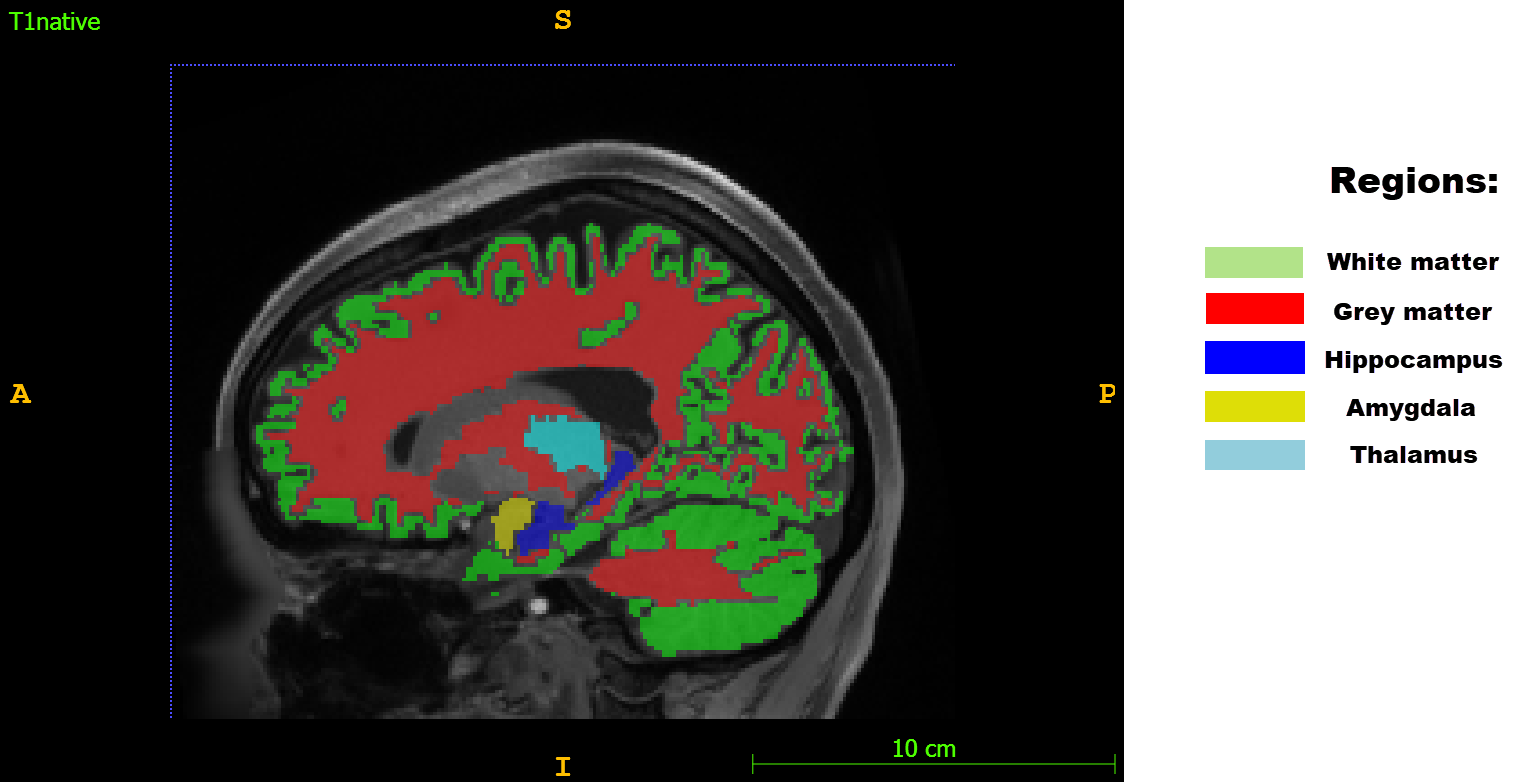
\includegraphics[width=0.5\textwidth]{T1native_all_regions_labelled.png}
		\caption{Ground truth picture of the five anatomibal brain regions to be segmented and labelled in this project.}
		\label{fig:e1}
	\end{figure}
	% --------------------------------------------------------------

\subsection{Data}
	The data used for this project was from the {\itshape Human Connectome Project} and has been provided by the Medical Image Analysis Lab team at the University of Bern. For anonymization the faces and ears of the skull have been blurred. 
	Overall, the dataset consisted of 30 MRI patient images of unrelated healthy subjects, out of which 20 were used for training and 10 for testing the model. 
	From each patient the ground truth image, the brain mask, a T1w and a T2w image were available. The images were generated by a 3 Tesla MRI. 
	The ground truth has been labelled by the silver standard and with the software FreeSurfer.
	The atlas used are the MNI152 standard-space T1-weighted average structural template images available from the {\itshape McConnell Brain Imaging Centre}\footnote{URL: \url{http://www.bic.mni.mcgill.ca/ServicesAtlases/HomePage}, Date: 23.12.2020.} (BIC) and the {\itshape NeuroImaging \& Surgical Technologies Lab}\footnote{URL: \url{http://nist.mni.mcgill.ca/?page_id=714}, Date: 23.12.2020. \label{second}}. 
	It corresponds to the MNI-ICBM atlas\footref{second} and is derived from 152 structural images, averaged together after high-dimensional nonlineal registration into this MNI152 coordinate system.
	Each MRI file is of the size 118x118x217 pixels.\smallskip
	The code was implemented in Python using scikit-learn \footnote{URL: \url{https://scikit-learn.org/stable/}, Date: 26.12.2020} and ITK\footnote{URL: \url{https://itk.org/}, Date: 26.12.2020}.
		
\subsection{Registration}
	During {\itshape Registration} the T1w and T2w image (floating image) is transformed with an affine transformation, such that it is similar to a given reference image.
	The transformation was found by an intersubjective registration from the T1w image to the provided atlas. The corresponding transformations have already been determined
	and are not part of this work. 	
	
\subsection{Preprocessing}
	The aim of {\itshape Pre-Processing} is to improve the image quality for the subsequent classification. It includes among others bias field correction, skull stripping, intensity normalization and/or histogram matching.
	Owing to the fact that the analysation and application of the impact of normalization to the realized segmentation, the used normalization techniques are described in this section.
	For this project the brain mask for skull stripping was provided. Skull stripping was performed before six different normalizations were applied to the image data. The results among all normalizations were compared to no-normalization. Primarily the used normalization methods are described. \cite{normalizations} \smallskip
		
	\subsubsection{ZScore}
	While the ZScore normalization the mean intensity value (mean) as well as the intensity standard deviation (istd) of all pixel values of the input image are calculated. 
	The image is normalized by subtracting the mean from each pixel value and then dividing this by the istd.
	This transforms the image data into an intensity distribution with a mean of 0 and a standard deviation of 1.
		\begin{equation}\label{ZScore}
			I_{New} = \frac{I - \mu}{\sigma}
		\end{equation}
			
	\subsubsection{MinMax}
	When applying the MinMax normalization method, the difference between the maximal and minimal intensity value (diff) of the input image is calculated. 
	Then the minimal intensity value of the image is subtracted from each pixel value. The result is then divided by the diff.
	This scales the intensities in a range from 0 to 1. 
		\begin{equation}
			I_{New} = \frac{I - I_{min}}{I_{max} - I_{min}}
		\end{equation}
		
	\subsubsection{Whitestripe}
	For the Whitestripe method equation \ref{ZScore} is likewise used. In contrast to the Z-Score normalization, $\mu$ and $\sigma$ are obtained from the intensity values of the normal appearing white matter (NAWM). 
	Thus, $\mu$ is obtained by smoothing the histogram and selecting the highest intensity peak. A 10\% segment around $\mu$ corresponds to the NAWM values of the T1w image. This segment is called the whitestripe.
	The standard deviation is then calculated from this whitestripe values.
	By applying the equation \ref{ZScore} with the obtained $\mu$ and $\sigma$ the peak of the white matter is shifted to 0 and the intensities are scaled with $\sigma$.
	\smallskip
		
	\subsubsection{Fuzzy C-Means}
	By using the Fuzzy C-Means algorithm, a mask of the white matter pixel values is created. 
	The obtained tissue mask is used to calculate the mean of all pixel intensity values of the white matter. This mean is called $\mu$.
	Following all image intensities are scaled by $\mu$ and shifted to a constant target value $c$.
		\begin{equation}
			I_{New} = \frac{c \cdot I}{\mu}
		\end{equation}
	
	\subsubsection{Gaussian Mixture Model}
	The Guassian Mixture Model normalization fits three Gaussian distributions to the skull stripped image intensity values. 
	The mean $\mu$ of the Gaussian distribution of the white matter is then used to normalize the image with the same equation \ref{FCM} as in the Fuzzy C-Means normalization method. 
	$c$ is again the target value where the mean $\mu$ is shifted to. 
	The mean $\mu$ in a T1w image corresponding to the white matter is the peak with the highest intensity values. 
	In a T2w image the white matter mean $\mu$ is the peak with the lowest intensity values. 
	\smallskip

	\subsubsection{Histogram Matching}
	Histogram matching manipulates the histogram of the input image in such a way that the histogram of the output image matches the histogram of a given reference image. 
	This is done by mapping the cumulative distribution function of the input image to the reference image.
	As a reference image the skull stripped T1w and T2w images of a subject were used. 
	\smallskip
	

\subsection{Feature Extraction \& Classifier} 
	The following seven features were being extracted: three Coordinate Features, a T1w and T2w Intensity Feature and a T1w and T2w Gradient Intensity Feature.\\
	The classifier used was a Random Forest classifier. It consists of numerous individual decision trees acting as an ensemble learning method for classification.
	The parameters to be chosen are the estimator and the tree depth. The estimator indicates the maximal number of decision trees. 
	The tree depth indicates the depth of each tree in the forest.
	This classifier tends to over-fit and caution has to be given when applying this classifier.
	After applying a grid search the parameters for the estimator=20 and the tree depth=190 were chosen. 
	
	
\subsection{Post-Processing} 
	To prevent any biases or interfering in the results and thus being able to better analyse the influence of the different normalizations, no post-processing methods were applied in this project. 
	
	
\subsection{Conducted experiment}
	To analyse the influence of the different normalizations, all parameters have been kept for all runs. 
	For each run, one out of the six normalization methods has been applied. One additional run has been conducted with no normalization method.
	To generate reproducible results the same random seed has been set for all runs.  
	
\subsection{Evaluation}
	To evaluate the segmentations obtained within this project the {\itshape Dice Similarity Coefficient} (DSC) as well as the {\itshape Hausdorff Distance} (HD) were applied.\\
	DSC returns a value between 0 and 1, indicating the percentage of overall pixels of the resulted segmentation (SEG) overlapping the ground truth (GT). 
	A result of 1 indicates a perfect segmentation. The equation states: 
	\begin{equation}
		DICE(SEG, GT) = 2 \frac{\mid SEG \cap GT \mid}{\mid SEG \mid + \mid GT \mid}
	\end{equation}

	The HD indicates whether the margin pixels of the obtain segmentation are close to the margin pixels of the ground truth. 
	The result is the largest distance of all pixels from one point in the segmentation to the closest point in the ground truth.
	The equation states:
	\begin{equation}
		d_H (SEG, GT) = \max \left\{ \underset{x\in SEG}{\mathop{\sup }}\,\underset{y\in GT}{\mathop{\inf }}\,d(x,y),\underset{y\in GT}{\mathop{\sup }}\,\underset{x\in SEG}{\mathop{\inf }}\,d(x,y) \right\}
	\end{equation}
	Because of sensitivity of outlier pixels, only the lowest 95\% percentile of HD values are taken into account.

	
%***************************************************************************************************************	

% --------------------------------------------------------------
% Results
% --------------------------------------------------------------

\section{Results}

	% --------------------------------------------------------------
	\begin{figure}[h]
		\centering
		%omit extension of file. pdflatex will convert to pdf automatically.
		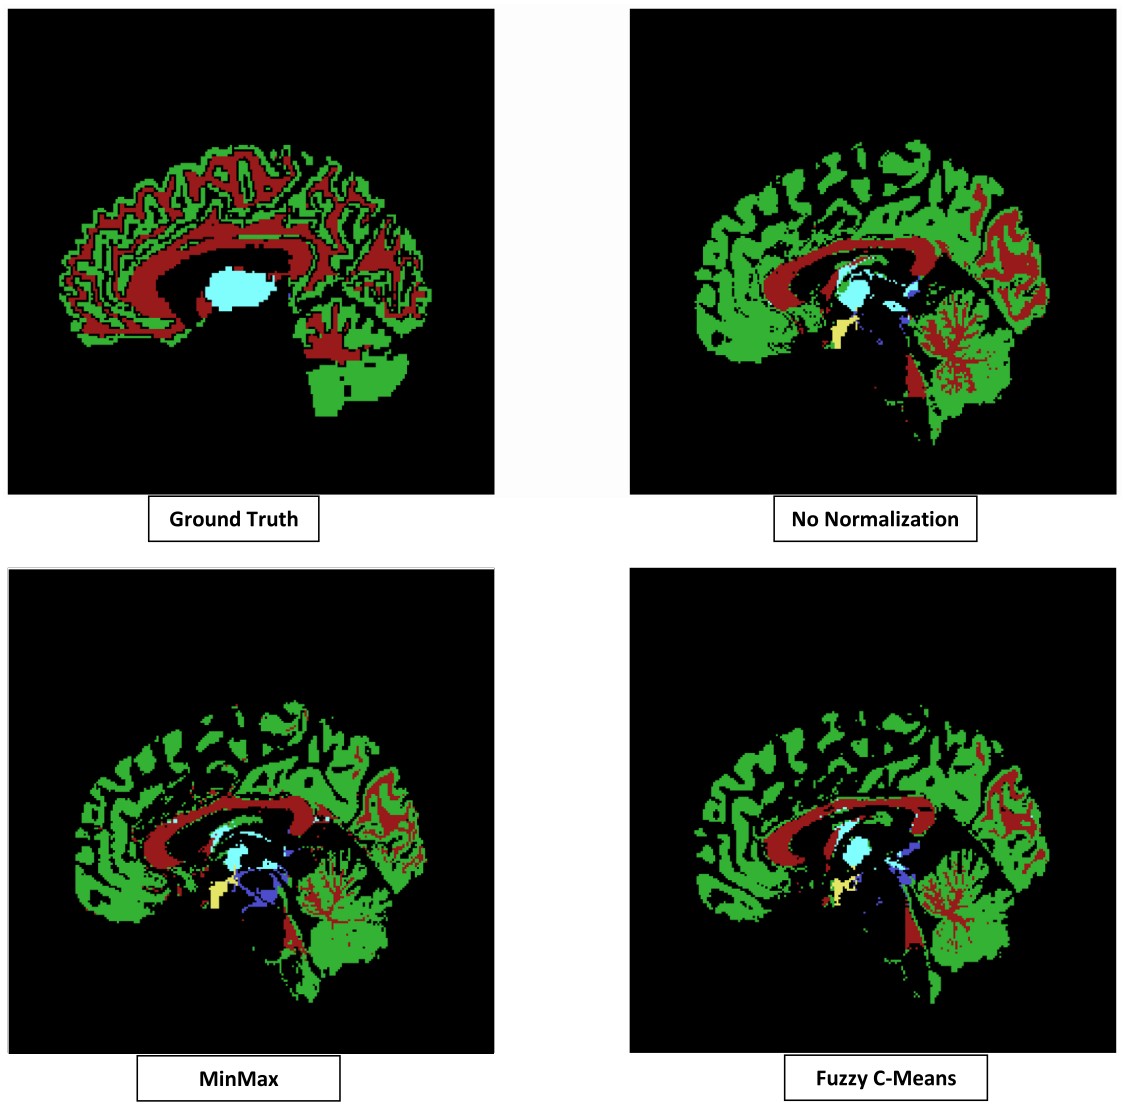
\includegraphics[width=0.5\textwidth]{compNorms.png}
		\caption{Comparison of no ground truth vs. different normalizations}
		\label{fig:e1}
	\end{figure}
	% --------------------------------------------------------------

An selection of results is depicted in Figure 3. Top left shows the ground-truth segmentation, so as similar our normalization look, the better.
Top right is the segmentation with no normalization and it is obvious that the result is much worse. The bottom row with MinMax ans Fuzzy C-Means
normalization look completely different than the ground truth as well, yet similar to no normalization. This suggests that there might be something wrong with
the algorithm already and that normalization has little to no effect. \\

Figure 4 depicts a similar suggestion.

% ----------------------------------------------------------------------------------------------------------------------------------------------------------------------------------------------------	
\begin{table}[h]
	\caption{The following table shows the results of all runs. In total there are seven runs, one without normalization and six with different normalization methods. The two metrics Dice coefficient (DC) and Hausdorff distance (HD) were obtained from the ten test subjects. The statistical values, mean $\mu$ and standard deviation $\sigma$, of DC and HD of the five segmented brain regions were determined.}
	\label{tab:diceHD}
	\begin{center}
	\begin{threeparttable}
	\begin{tabular}{c c c c c c c}
		\toprule
			\textbf{Normalization} & \textbf{Metric} &  \textbf{Thalamus} & \textbf{White Matter} & \textbf{Grey Matter} & \textbf{Amygdala} & \textbf{Hippocampus} \\ \midrule
		No Normalization		&	DC	&	$\mu$: 0.64, $\sigma$: 0.04		&	$\mu$: 0.65, $\sigma$: 0.06		&	$\mu$: 0.39, $\sigma$: 0.02		&	$\mu$: 0.37, $\sigma$: 0.07		&	$\mu$: 0.24, $\sigma$: 0.02		\\ \cmidrule(lr{1em}){2-7}
								&	HD	&	$\mu$: 24.58, $\sigma$: 15.70	&	$\mu$: 4.94, $\sigma$: 0.71		&	$\mu$: 5.41, $\sigma$: 1.46		&	$\mu$: 18.58, $\sigma$: 4.59	&	$\mu$: 22.31, $\sigma$: 3.04	\\ \midrule
		ZScore					&	DC	&	$\mu$: 0.64, $\sigma$: 0.02		&	$\mu$: 0.67, $\sigma$: 0.03		&	$\mu$: 0.40, $\sigma$: 0.02		&	$\mu$: 0.37, $\sigma$: 0.04		&	$\mu$: 0.26, $\sigma$: 0.01 	\\ \cmidrule(lr{1em}){2-7}
								&	HD	&	$\mu$: 39.27, $\sigma$: 2.36	&	$\mu$: 4.24, $\sigma$: 0.35		&	$\mu$: 4.60, $\sigma$: 0.57		&	$\mu$: 15.82, $\sigma$: 0.92	&	$\mu$: 20.65, $\sigma$: 0.86 	\\ \midrule
		MinMax 					&	DC	&	$\mu$: 0.66, $\sigma$: 0.03		&	$\mu$: 0.65, $\sigma$: 0.03		&	$\mu$: 0.39, $\sigma$: 0.02		&	$\mu$: 0.37, $\sigma$: 0.04		&	$\mu$: 0.24, $\sigma$: 0.02 	\\ \cmidrule(lr{1em}){2-7}
								&	HD	&	$\mu$: 21.04, $\sigma$: 1.73	&	$\mu$: 5.53, $\sigma$: 0.31		&	$\mu$: 5.04, $\sigma$: 0.92		&	$\mu$: 17.45, $\sigma$: 0.72	&	$\mu$: 20.43, $\sigma$: 1.63 	\\ \midrule
		Whitestripe 			&	DC	&	$\mu$: 0.60, $\sigma$: 0.17		&	$\mu$: 0.64, $\sigma$: 0.09		&	$\mu$: 0.39, $\sigma$: 0.02		&	$\mu$: 0.37, $\sigma$: 0.03		&	$\mu$: 0.25, $\sigma$: 0.01 	\\ \cmidrule(lr{1em}){2-7}
								&	HD	&	$\mu$: 38.19, $\sigma$: 5.74	&	$\mu$: 4.39, $\sigma$: 0.30		&	$\mu$: 4.78, $\sigma$: 0.99		&	$\mu$: 20.10, $\sigma$: 5.33	&	$\mu$: 22.24, $\sigma$: 3.80 	\\ \midrule
		Fuzzy C-Means 			&	DC	&	$\mu$: 0.61, $\sigma$: 0.03		&	$\mu$: 0.68, $\sigma$: 0.03		&	$\mu$: 0.40, $\sigma$: 0.02		&	$\mu$: 0.39, $\sigma$: 0.03		&	$\mu$: 0.26, $\sigma$: 0.01 	\\ \cmidrule(lr{1em}){2-7}
								&	HD	&	$\mu$: 41.41, $\sigma$: 0.64	&	$\mu$: 4.01, $\sigma$: 0.33		&	$\mu$: 4.80, $\sigma$: 0.67		&	$\mu$: 17.46, $\sigma$: 2.41	&	$\mu$: 20.35, $\sigma$: 1.15 	\\ \midrule
		Gaussian Mixture Model 	&	DC	&	$\mu$: 0.67, $\sigma$: 0.03		&	$\mu$: 0.68, $\sigma$: 0.02 	& 	$\mu$: 0.42, $\sigma$: 0.02		& 	$\mu$: 0.41, $\sigma$: 0.03 	& 	$\mu$: 0.39, $\sigma$: 0.01 	\\ \cmidrule(lr{1em}){2-7}
								&	HD	& 	$\mu$: 38.06, $\sigma$: 1.14 	& 	$\mu$: 4.08, $\sigma$: 0.17 	& 	$\mu$: 3.38, $\sigma$: 0.29 	& 	$\mu$: 17.34, $\sigma$: 3.63 	& 	$\mu$: 17.57, $\sigma$: 1.83 	\\ \midrule
		Histogram Matching	 	&	DC	& 	$\mu$:0.65, $\sigma$: 0.02 		& 	$\mu$: 0.61, $\sigma$: 0.04 	& 	$\mu$: 0.42, $\sigma$: 0.02 	& 	$\mu$: 0.42, $\sigma$: 0.04		& 	$\mu$: 0.28, $\sigma$: 0.02 	\\ \cmidrule(lr{1em}){2-7}
								&	HD	& 	$\mu$: 23.26, $\sigma$: 1.29	&  	$\mu$: 5.91, $\sigma$: 0.38 	& 	$\mu$: 3.06, $\sigma$: 0.17 	& 	$\mu$: 17.25, $\sigma$: 2.27	& 	$\mu$: 28.37, $\sigma$: 2.20 	\\  \bottomrule
	\end{tabular}
	\end{threeparttable}
	\end{center}
	\label{table:simDisimCoefNewDef}
	\end{table}
	% ----------------------------------------------------------------------------------------------------------------------------------------------------------------------------------------------------

% --------------------------------------------------------------
% Discussion
% --------------------------------------------------------------

\section{Discussion}
\textbf{Aims of the Discussion part:
\begin{itemize}
\item Highlight importance of your work (highlight novelty /impact etc
\item To interpret your results in relation to your original problem
\item To put your work into the context of existing work
\item To present any limitations of the presented work
\item To make future recommendations
\item To provide a conclusion of the work
\end{itemize}
\begin{enumerate}
\item Importance of the work
	\begin{enumerate}
	\item Summarise your results
	\item Reiterate the importance of the work (novelty , impact etc)
	\end{enumerate}
\item Interpretation of results
	\begin{enumerate}
	\item Interpret your results focussing on the problem described in the introduction. What do the results mean for the described problem?
	\item Explain any unusual/important findings (be careful if not your original investigative subject)
	\end{enumerate}
\item Provide context
	\begin{enumerate}
	\item Describe your results in relation to others and try to explain any discrepancies
	\item Emphasize how your results support or refute your hypotheses current thinking in the field. Were results as expected? If not why and what does this mean?
	\end{enumerate}
\item Limitations of your work
	\begin{enumerate}
	\item Describe any limitations /deficiencies of your work and what impact they have on the findings
	\item Suggest possible future solutions
	\end{enumerate}
\end{enumerate} 
}

% --------------------------------------------------------------
% Conclusion
% --------------------------------------------------------------

\section{Conclusion}
\textbf{	
	\begin{itemize}
	\item Summarise your findings and relate your findings back to your hypothesis / aim / objective and to your problem.
	\item Based on your findings, suggest next steps towards solving your problem
	\end{itemize}
}
\pagebreak

% --------------------------------------------------------------
% References
% --------------------------------------------------------------

\bibliographystyle{ieeetr}
\bibliography{MIALab} 

\end{document}
